\subsection{Упражнение 1}

Изучим влияние diff и differentiate на сигнал. Создадим треугольный сигнал.

\begin{lstlisting}[language=Python]
from thinkdsp import TriangleSignal

wave = TriangleSignal(freq=40).make_wave(duration=0.2, framerate=44100)
wave.plot()
decorate(xlabel='Time (s)')
\end{lstlisting}

\begin{figure}[H]
	\begin{center}
		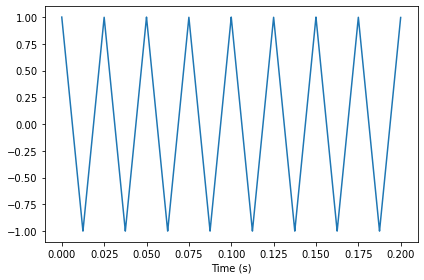
\includegraphics[scale=1]{fig/lab09/lab09_01.png}
		\caption{График сигнала}
	\end{center}
\end{figure}

Функция diff

\begin{lstlisting}[language=Python]
wave_diff = wave.diff()
wave_diff.plot()
decorate(xlabel='Time (s)')
\end{lstlisting}

\begin{figure}[H]
	\begin{center}
		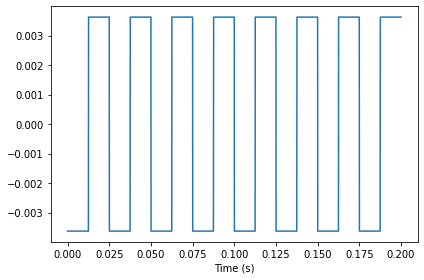
\includegraphics[scale=1]{fig/lab09/lab09_02.png}
		\caption{Сигнал после применения diff}
	\end{center}
\end{figure}

Функция differentiate

\begin{lstlisting}[language=Python]
wave_differentiate = wave.make_spectrum().differentiate().make_wave()
wave_differentiate.plot()
decorate(xlabel='Time (s)')
\end{lstlisting}

\begin{figure}[H]
	\begin{center}
		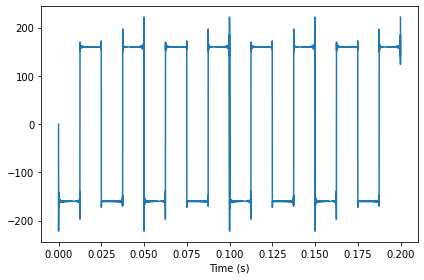
\includegraphics[scale=1]{fig/lab09/lab09_03.png}
		\caption{Сигнал после применения differentiate}
	\end{center}
\end{figure}

Видны различия в местах перегиба

\subsection{Упражнение 2}

Испытаем cumsum и integrate на прямоугольном сигнале

\begin{lstlisting}[language=Python]
from thinkdsp import SquareSignal

wave = SquareSignal(freq=40).make_wave(duration=0.2, framerate=44100)
wave.plot()
decorate(xlabel='Time (s)')
\end{lstlisting}

\begin{figure}[H]
	\begin{center}
		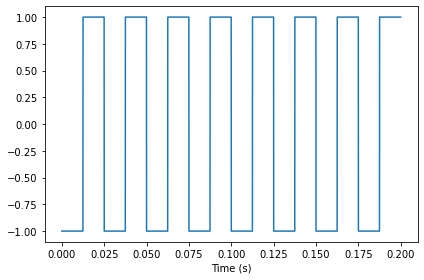
\includegraphics[scale=1]{fig/lab09/lab09_04.png}
		\caption{Рассматриваемый сигнал}
	\end{center}
\end{figure}

cumsum

\begin{lstlisting}[language=Python]
wave_cumsum = wave.cumsum()
wave_cumsum.plot()
decorate(xlabel='Time (s)')
\end{lstlisting}

\begin{figure}[H]
	\begin{center}
		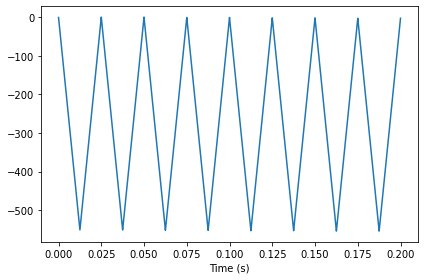
\includegraphics[scale=1]{fig/lab09/lab09_05.png}
		\caption{Рассматриваемый сигнал после применения cumsum}
	\end{center}
\end{figure}

Получился треугольный сигнал, так как мы аппроксимировали интегрирование.

Используем integrate на спектре и обратно перобразуем в волну

\begin{lstlisting}[language=Python]
spectrum = wave.make_spectrum().integrate()
spectrum.hs[0] = 0
wave_spectrum = spectrum.make_wave()
wave_spectrum.plot()
decorate(xlabel='Time (s)')
\end{lstlisting}

\begin{figure}[H]
	\begin{center}
		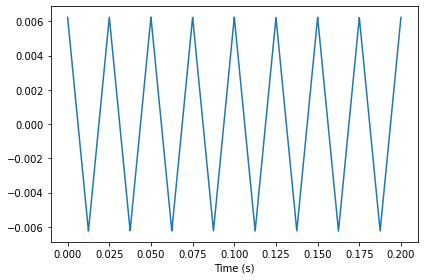
\includegraphics[scale=1]{fig/lab09/lab09_06.png}
		\caption{Рассматриваемый сигнал после применения integrate}
	\end{center}
\end{figure}

Отличия только в амплитуде


\subsection{Упражнение 3}

Посмотрим на двойное интегрирование пилообразного сигнала

\begin{lstlisting}[language=Python]
from thinkdsp import SawtoothSignal

wave = SawtoothSignal(freq=40).make_wave(duration=0.2, framerate=44100)
wave.plot()
decorate(xlabel='Time (s)')
\end{lstlisting}

\begin{figure}[H]
	\begin{center}
		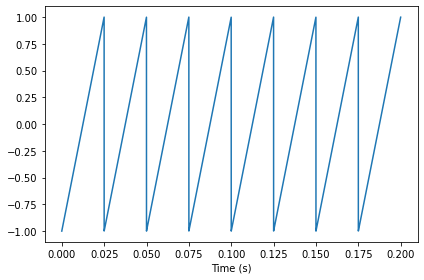
\includegraphics[scale=1]{fig/lab09/lab09_07.png}
		\caption{Пилообразный сигнал}
	\end{center}
\end{figure}


\begin{lstlisting}[language=Python]
spectrum = wave.make_spectrum().integrate().integrate()
spectrum.hs[0] = 0

wave_out = spectrum.make_wave()
wave_out.plot()
decorate(xlabel='Time (s)')
\end{lstlisting}

\begin{figure}[H]
	\begin{center}
		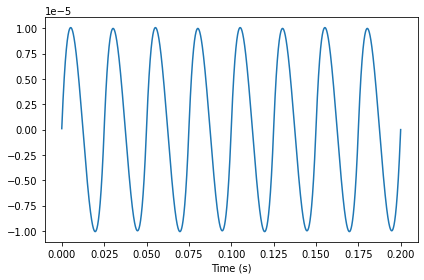
\includegraphics[scale=1]{fig/lab09/lab09_08.png}
		\caption{Двойное интегрирование}
	\end{center}
\end{figure}

Получили кубическую кривую, который похож на синусоиду, двойное интегрирование действует как фильтр нижних частот.

\begin{lstlisting}[language=Python]
wave_out.make_spectrum().plot(high=500)
\end{lstlisting}

\begin{figure}[H]
	\begin{center}
		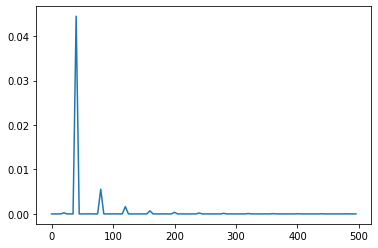
\includegraphics[scale=1]{fig/lab09/lab09_09.png}
		\caption{График}
	\end{center}
\end{figure}


\subsection{Упражнение 4}

Проверм влияние второй разности и второй производной на CubicSignal

\begin{lstlisting}[language=Python]
from thinkdsp import CubicSignal

wave = CubicSignal(freq=0.0005).make_wave(duration=10000, framerate=1)
wave.plot()
\end{lstlisting}

\begin{figure}[H]
	\begin{center}
		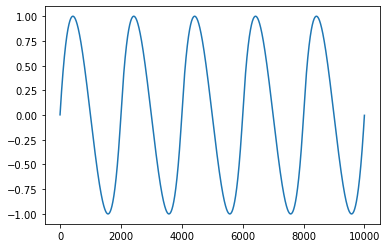
\includegraphics[scale=1]{fig/lab09/lab09_10.png}
		\caption{Кубический сигнал}
	\end{center}
\end{figure}


\begin{lstlisting}[language=Python]
wave_diff_1 = wave.diff()
wave_diff_1.plot()
\end{lstlisting}

\begin{figure}[H]
	\begin{center}
		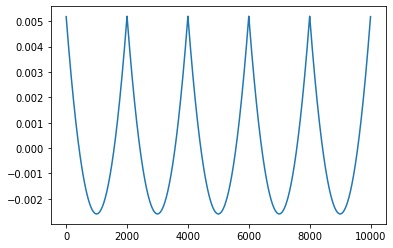
\includegraphics[scale=1]{fig/lab09/lab09_11.png}
		\caption{Первая разность}
	\end{center}
\end{figure}

\begin{lstlisting}[language=Python]
wave_diff_2 = wave_diff_1.diff()
wave_diff_2.plot()
\end{lstlisting}

\begin{figure}[H]
	\begin{center}
		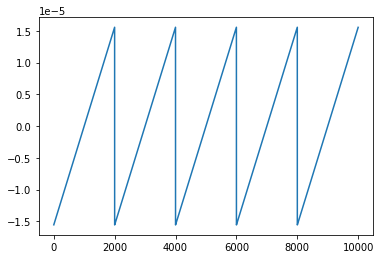
\includegraphics[scale=1]{fig/lab09/lab09_12.png}
		\caption{Вторая разность}
	\end{center}
\end{figure}

Первая разность - это парабола, а вторая разность - пилообразный сигнал

\begin{lstlisting}[language=Python]
spectrum = wave.make_spectrum().differentiate().differentiate()
wave_differentiate = spectrum.make_wave()
wave_differentiate.plot()
decorate(xlabel='Time (s)')
\end{lstlisting}

\begin{figure}[H]
	\begin{center}
		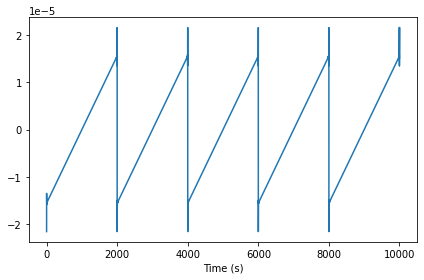
\includegraphics[scale=1]{fig/lab09/lab09_13.png}
		\caption{Полученный сигнал со звоном}
	\end{center}
\end{figure}
После двойного дифференцирования differentiate на графике виден пилообразный сигнал с звоном, из-за того, что производная параболического сигнала в некоторых точках не определена.

Окно второй разности это -1, 2, -1. При вычислении ДПФ можно найти соответствующий фильтр.

\begin{lstlisting}[language=Python]
from thinkdsp import zero_pad
from thinkdsp import Wave

diff_window = np.array([-1.0, 2.0, -1.0])
padded = zero_pad(diff_window, len(wave))
diff_wave = Wave(padded, framerate=wave.framerate)
diff_filter = diff_wave.make_spectrum()
diff_filter.plot(label='2nd diff')

decorate(xlabel='Frequency (Hz)',
                 ylabel='Amplitude ratio')
\end{lstlisting}

\begin{figure}[H]
	\begin{center}
		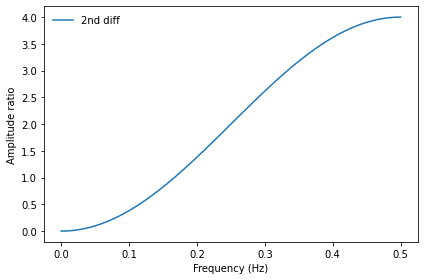
\includegraphics[scale=1]{fig/lab09/lab09_14.png}
		\caption{Первый фильтр}
	\end{center}
\end{figure}

Для второй производной можно найти соответствующий фильтр, рассчитав фильтр первой производной и возведя его в квадрат:

\begin{lstlisting}[language=Python]
deriv_filter = wave.make_spectrum()
deriv_filter.hs = (2 * np.pi * 1j * deriv_filter.fs)**2
deriv_filter.plot()
\end{lstlisting}

\begin{figure}[H]
	\begin{center}
		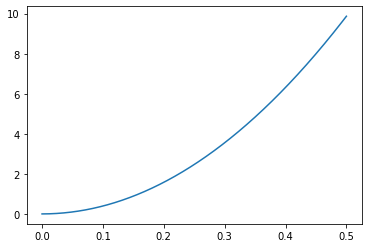
\includegraphics[scale=1]{fig/lab09/lab09_15.png}
		\caption{Второй фильтр}
	\end{center}
\end{figure}

Сравним эти два графика

\begin{lstlisting}[language=Python]
diff_filter.plot(label='2nd diff')
deriv_filter.plot(label='2nd deriv')

decorate(xlabel='Frequency (Hz)',
                 ylabel='Amplitude ratio')
\end{lstlisting}

\begin{figure}[H]
	\begin{center}
		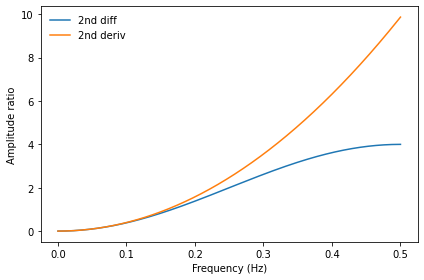
\includegraphics[scale=1]{fig/lab09/lab09_16.png}
		\caption{Сравнение фильтров}
	\end{center}
\end{figure}

Оба являются фильтрами верхних частот, которые усиливают высокочастотные компоненты. Вторая производная является параболической, поэтому она больше всего усиливает самые высокие частоты, а вторая разность является хорошей аппроксимацией второй производной только на самых низких частотах, далее она существенно отклоняется.


\subsection{Вывод}

В данной работе были рассмотрены соотношения между окнами во временной области и фильтрами в частотной. Были рассмотрены конечные разности, аппроксимирующее дифференцирование и накапливающие суммы с аппроксимирующим интегрированием.